\chapter{Keypoint Detection}
(Corner Detection)

\begin{introduction}[Keywords]
    \item 角点检测 Corner Detection
    \item 结构张量 Structure Tensor
    \item 特征值分解 Eigenvalue Decomposition
    \item 等变性 Equivariance
    \item 尺度不变性 Scale Invariance
    \item Harris-Laplacian 检测器
    \item 高斯差分 Difference-of-Gaussians (DoG)
\end{introduction}

\begin{problem}
    What Points are Keypoints?
\end{problem}

\begin{enumerate}
    \item Repeatability: 可以在不同的图像中找到相同的点
    \item Saliency: 有趣的点
    \item Quantity: 量大管饱
    \item Accurate localization: 精确定位
\end{enumerate}
Corners 就是这样的 keypoints.




\section{The Basic Idea of Harris Corner}

\begin{figure}[htbp]
    \centering
    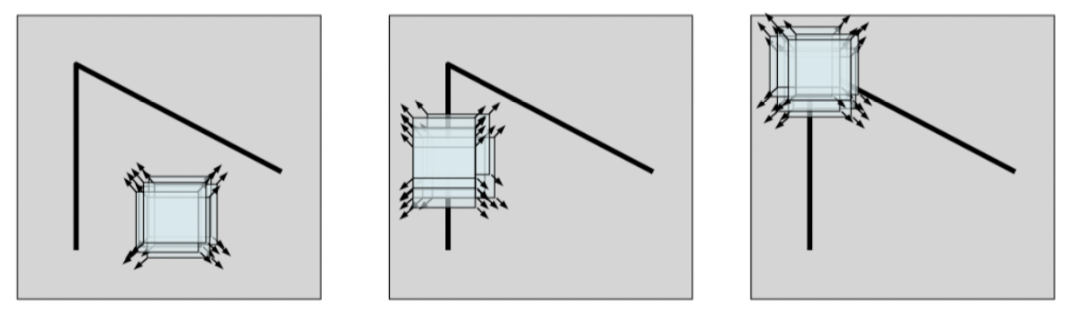
\includegraphics[width=0.8\textwidth]{figures/window_moving.png}
    \caption{移动窗口}    
\end{figure}

Move a window and explore intensity changes within the window.

Corner : significant change in all directions.

\section{Harris Corner}

一个 window,给定它的移动方向 $(u,v)$:

\begin{equation}
    \begin{aligned}
    E(u,v) &= \sum_{x,y} w(x,y) [I(x+u,y+v) - I(x,y)]^2\\
    &\approx \sum_{x,y} w(x,y) [I(x,y) + uI_x + vI_y - I(x,y)]^2\\
    &= \sum_{x,y} w(x,y) [uI_x + vI_y]^2\\
    &= w \ast \begin{bmatrix} u & v \end{bmatrix} \begin{bmatrix} I_x^2 & I_xI_y \\ I_xI_y & I_y^2 \end{bmatrix} \begin{bmatrix} u \\ v \end{bmatrix}\\
    &= \begin{bmatrix} u & v \end{bmatrix} \begin{bmatrix} w \ast I_x^2 & w \ast I_xI_y \\ w \ast I_xI_y & w \ast I_y^2 \end{bmatrix} \begin{bmatrix} u \\ v \end{bmatrix}\\
    &= \begin{bmatrix} u & v \end{bmatrix} R^{-1} \begin{bmatrix} \lambda_1 & 0\\ 0 & \lambda_2 \end{bmatrix} R \begin{bmatrix} u \\ v \end{bmatrix}\\
    &= \lambda_1 u_R^2 + \lambda_2 v_R^2
    \end{aligned}
\end{equation}

根据这两个特征值的大小可以判断这个点是不是角点.

\begin{figure}[htbp]
    \centering
    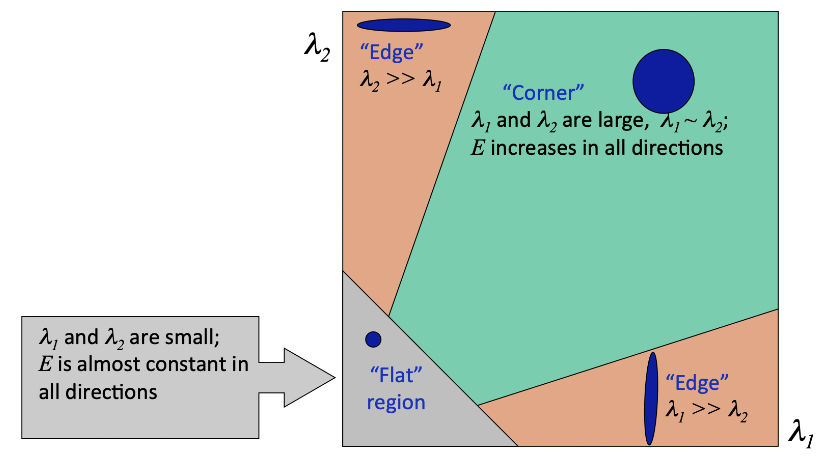
\includegraphics[width=0.6\textwidth]{figures/corner_map.png}
    \caption{特征值大小和这个点的是什么种类的点的关系}
\end{figure}
\begin{proposition}
    

这个点是角点一般需要满足:

\begin{itemize}
    \item $\lambda_1, \lambda_2>b$
    \item $\frac{1}{k}<\frac{\lambda_1}{\lambda_2}<k$
\end{itemize}

一个快速的判断公式:

\begin{equation}
\begin{aligned}
\theta&=\frac 12(\lambda_1\lambda_2-\alpha(\lambda_1+\lambda_2)^2)+\frac12(\lambda_1\lambda_2-2t)\\
&=\lambda_1\lambda_2-\alpha(\lambda_1+\lambda_2)^2-t\\
&=\det(R)-\alpha\text{Trace}(R)^2-t
\end{aligned}
\end{equation}

其中 $\alpha\in[0.04,0.06], t\in[0.01,0.03]$.

如果 $\theta$ 大于阈值, 则认为这个点是角点.
\end{proposition}
\begin{note}
Harris Corner 对平移和图像旋转是 equivariant的,对规模不是 equivariant 的.

为实现 rotation invariance, 可以用 Gaussian filter 来平滑图像, 使得角点不会因为旋转而改变.
\end{note}
\section{equivariant V.S. invariant}
\begin{definition}
    

\textbf{等变 (equivariant)}: $F(TX)=T(F(x))$,对于translation和rotation是等变的.

\textbf{不变 (invariant)}: $F(T(X))=F(X)$,也就是对于不同位置导出的角点还是那样,所以其实我们想要的是等变,也就是对于不同位置导出的角点做了同样的变化.
\end{definition}

\begin{problem}
    How to prove Harris detector is equivariant?
\end{problem}


只要说明角点检测函数也是equivariant即可.

角点检测函数包括了求导和卷积两个操作,显然求导是equivariant的,因为导数会随着trans和rot做相同的变化.

很有趣的是卷积也是equivariant的:当你的filter function是各向同性的,那么这个卷积就是equivariant的;但是如果是一个椭圆形的window,那这个卷积就不是equivariant的了.

\begin{figure}[htbp]
    \centering
    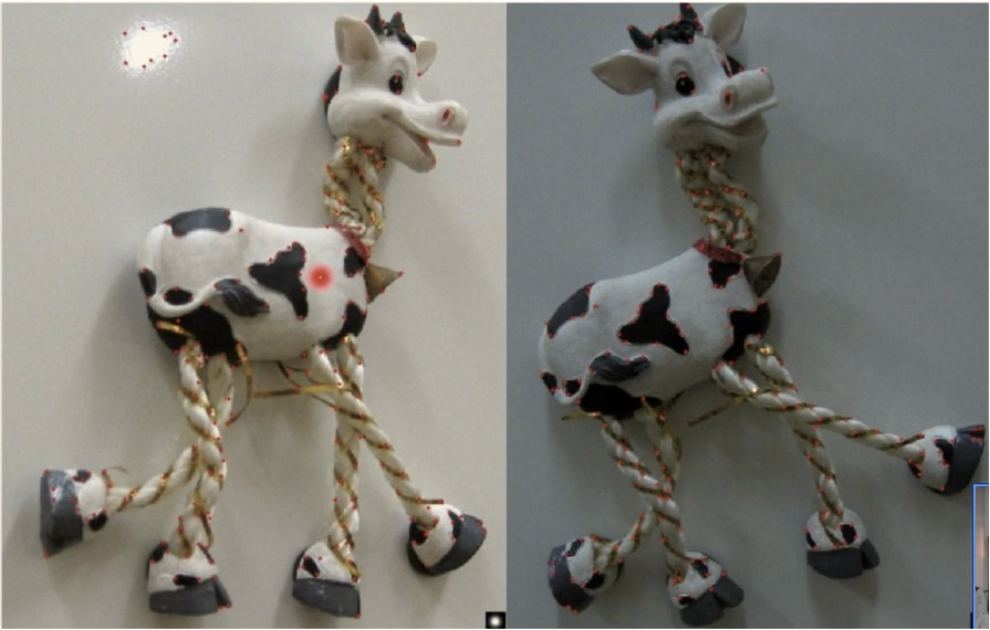
\includegraphics[width=0.6\textwidth]{figures/light_invariant.png}
    \caption{Illumination invariant}
\end{figure}
\begin{remark}
    这个高光说明不是环境 Illumination Invariant的
\end{remark}


\begin{problem}
    How to do NMS with corner-response-function?
\end{problem}


一个简单的想法:

先给出一个阈值,把所有response排序,成为一个list,从上到下按顺序把这个pixel周围的大于阈值的踢出list.
这个跟之前的NMS区别在于之前需要一条边,现在只需要一个点,那么现在比之前踢出的像素点更多.

\section{Scale Invariant Detectors}

这个不讲了?下次看看

Harris-Laplacian, SIFT (Lowe)